

\documentclass[10pt,red]{beamer} 
% change the alerted colour to blue
\setbeamercolor{alerted text}{fg=blue}

\usetheme{berlin}
% theme split
\usepackage{beamerthemesplit}

\usepackage{booktabs,array,}
\usepackage{listings}
\usepackage{hyperref}
\usepackage{verbatim,moreverb}
\usepackage{tikz}

\usepackage{color}

\definecolor{dkgreen}{rgb}{0,0.6,0}
\definecolor{gray}{rgb}{0.5,0.5,0.5}
\definecolor{mauve}{rgb}{0.58,0,0.82}

\lstset{frame=tb,
  language = Java,
  aboveskip=3mm,
  belowskip=3mm,
  showstringspaces=true,
  columns=flexible,
  basicstyle={\small\ttfamily},
  numbers=none,
  numberstyle=\tiny\color{gray},
  keywordstyle=\color{blue},
  commentstyle=\color{dkgreen},
  stringstyle=\color{mauve},
  breaklines=true,
  breakatwhitespace=true
  tabsize=4
}
% theme shadow
\usepackage{beamerthemeshadow}

% For including figures
\usepackage{graphicx}

% logo
\logo{
\includegraphics[height=1cm]{iitblogo.pdf}}


% sf family, bold font
\sffamily \bfseries
% Beginning of title page
\title
% content inside [] appears at bottom of all page. content inside {} appears on first page as title. double backslash means line change 
[
	Raspberry Pi Hardware Development	% bottom
	\hspace{0.5cm}
	\insertframenumber/\inserttotalframenumber
]
{
	Accessing GPIO pins on Raspberry Pi
}

\author
[
	www.e-yantra.org
]
{
	e-Yantra Team \\
  Embedded Real-Time Systems Lab\\
  Indian Institute of Technology-Bombay \\
}
\date
{
IIT Bombay \\ {\today}
}
 
 
\begin{document} 

% Slide-1: Title Page
\begin{frame}
	\titlepage
\end{frame} 

\section{GPIO pins on RPi}
\subsection{Overview of GPIO pins}
% Slide-3: Definition of PORTs
\begin{frame}
	\frametitle{What is GPIO?} \pause
		\begin{enumerate}
			\item<+-|alert@+> Stands for General Purpose Input Output where external hardware can be connected \\[10pt]
			\item<+-|alert@+> The external hardware can be the input or output device  \\[10pt]
				\begin{itemize}
				\item<+-|alert@+> Input Device  \\[10pt]
				 Example: Switch, Sensors, Keyboard etc...\\[10pt]
				 \item<+-|alert@+> Output Device  \\[10pt]
				 Example: Buzzer, LCD, Motors, LED etc...    
				\end{itemize}
		\end{enumerate}
\end{frame}

\begin{frame}
	\frametitle{Raspberry Pi Pinouts} \pause
	\centering
	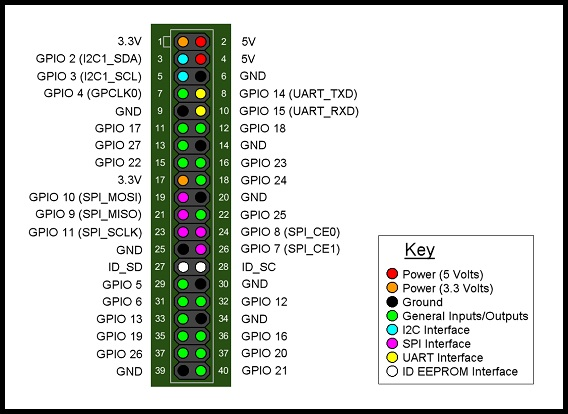
\includegraphics[scale= 0.4]{rpi_pinout.jpg}
\end{frame}
\begin{frame}
	\frametitle{Experiment} \pause
	\textbf{Interfacing an LED with the Raspberry Pi.}
\end{frame}
\section{Write Your First Python Program}
\subsection{Led Interfacing}
\begin{frame}
	\frametitle{Hardware Required for the experiments:}	\pause
		\begin{enumerate}
			\item<+-|alert@+> Breadboard 	
			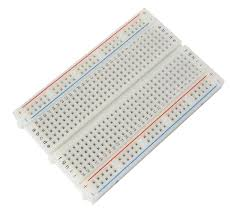
\includegraphics[scale=0.3]{breadboard}
			\item<+-|alert@+>  LED
			
\includegraphics[scale=0.2]{led}
			\item<+-|alert@+> 330 ohm resistor
			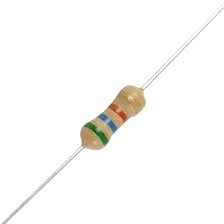
\includegraphics[scale=0.1]{resistor}
			
		\end{enumerate}
\end{frame}
\subsection{Connections}
\begin{frame}
	\frametitle{Connections:}
	\begin{enumerate}
		\item<+-|alert@+> Anode of the LED is connected to pin no. 35 (i.e. GPIO 19 pin)
		\item<+-|alert@+> Cathode of the LED is connected to a resistor(330 ohms) which is in turn connected to GND pin on R-Pi.
	\end{enumerate}
\end{frame}
\begin{frame}
	\begin{enumerate}
	\item	Figure shows the connections of LED and Raspberry Pi.
	\vspace{5mm}
	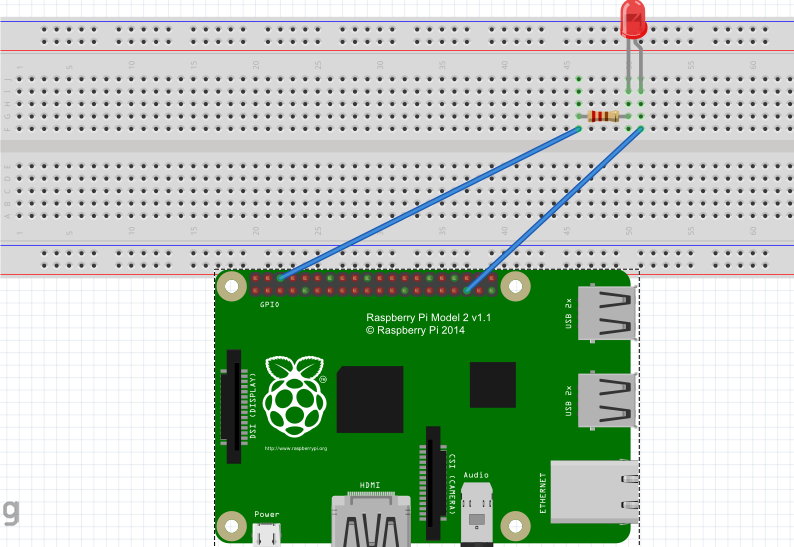
\includegraphics[scale=0.4]{gpio.png}
	\end{enumerate}	
\end{frame}
\subsection{Problem Statement}
\begin{frame}
	\frametitle{Problem Statement}
	\textbf{Turn on the LED for 1 second and then turn it off for 1 second and repeat the process continuously.}
\end{frame}
\begin{frame}
	\frametitle{Exercise} \pause
	\textbf{Controlling a led using a push button}
\end{frame}
\begin{frame}
\hskip4cm
\textbf{\LARGE Thank You!} \\[20pt]
\hskip3cm
\scriptsize Post your queries on: 
\hyperref[www.e-yantra.org]{\color{blue} http://qa.e-yantra.org/ \color{black}} 
\end{frame}
\end{document} 